\chapter{Matching}

\begin{descr}
    Matchings in undirected graphs without parallel edges and loops
\end{descr}

\section{Elementary Definitions}\index{Elementary Definitions}
\begin{definition}
A matching in an undirected (finite) graph $G=(V,E)$ is a set $M \subseteq E$ such that no two edges share a node.
A matching $M$ is called \emph{maximal} if, for any matching $M'$ with $M \subseteq M'$, $M=M'$ holds.
$M$ is of maximum cardinality if $\lvert M \rvert \ge \lvert M' \rvert $ for any matching $M'$. $M$ is \emph{perfect}
if every node is incident on one edge.
\end{definition}

\begin{example*}
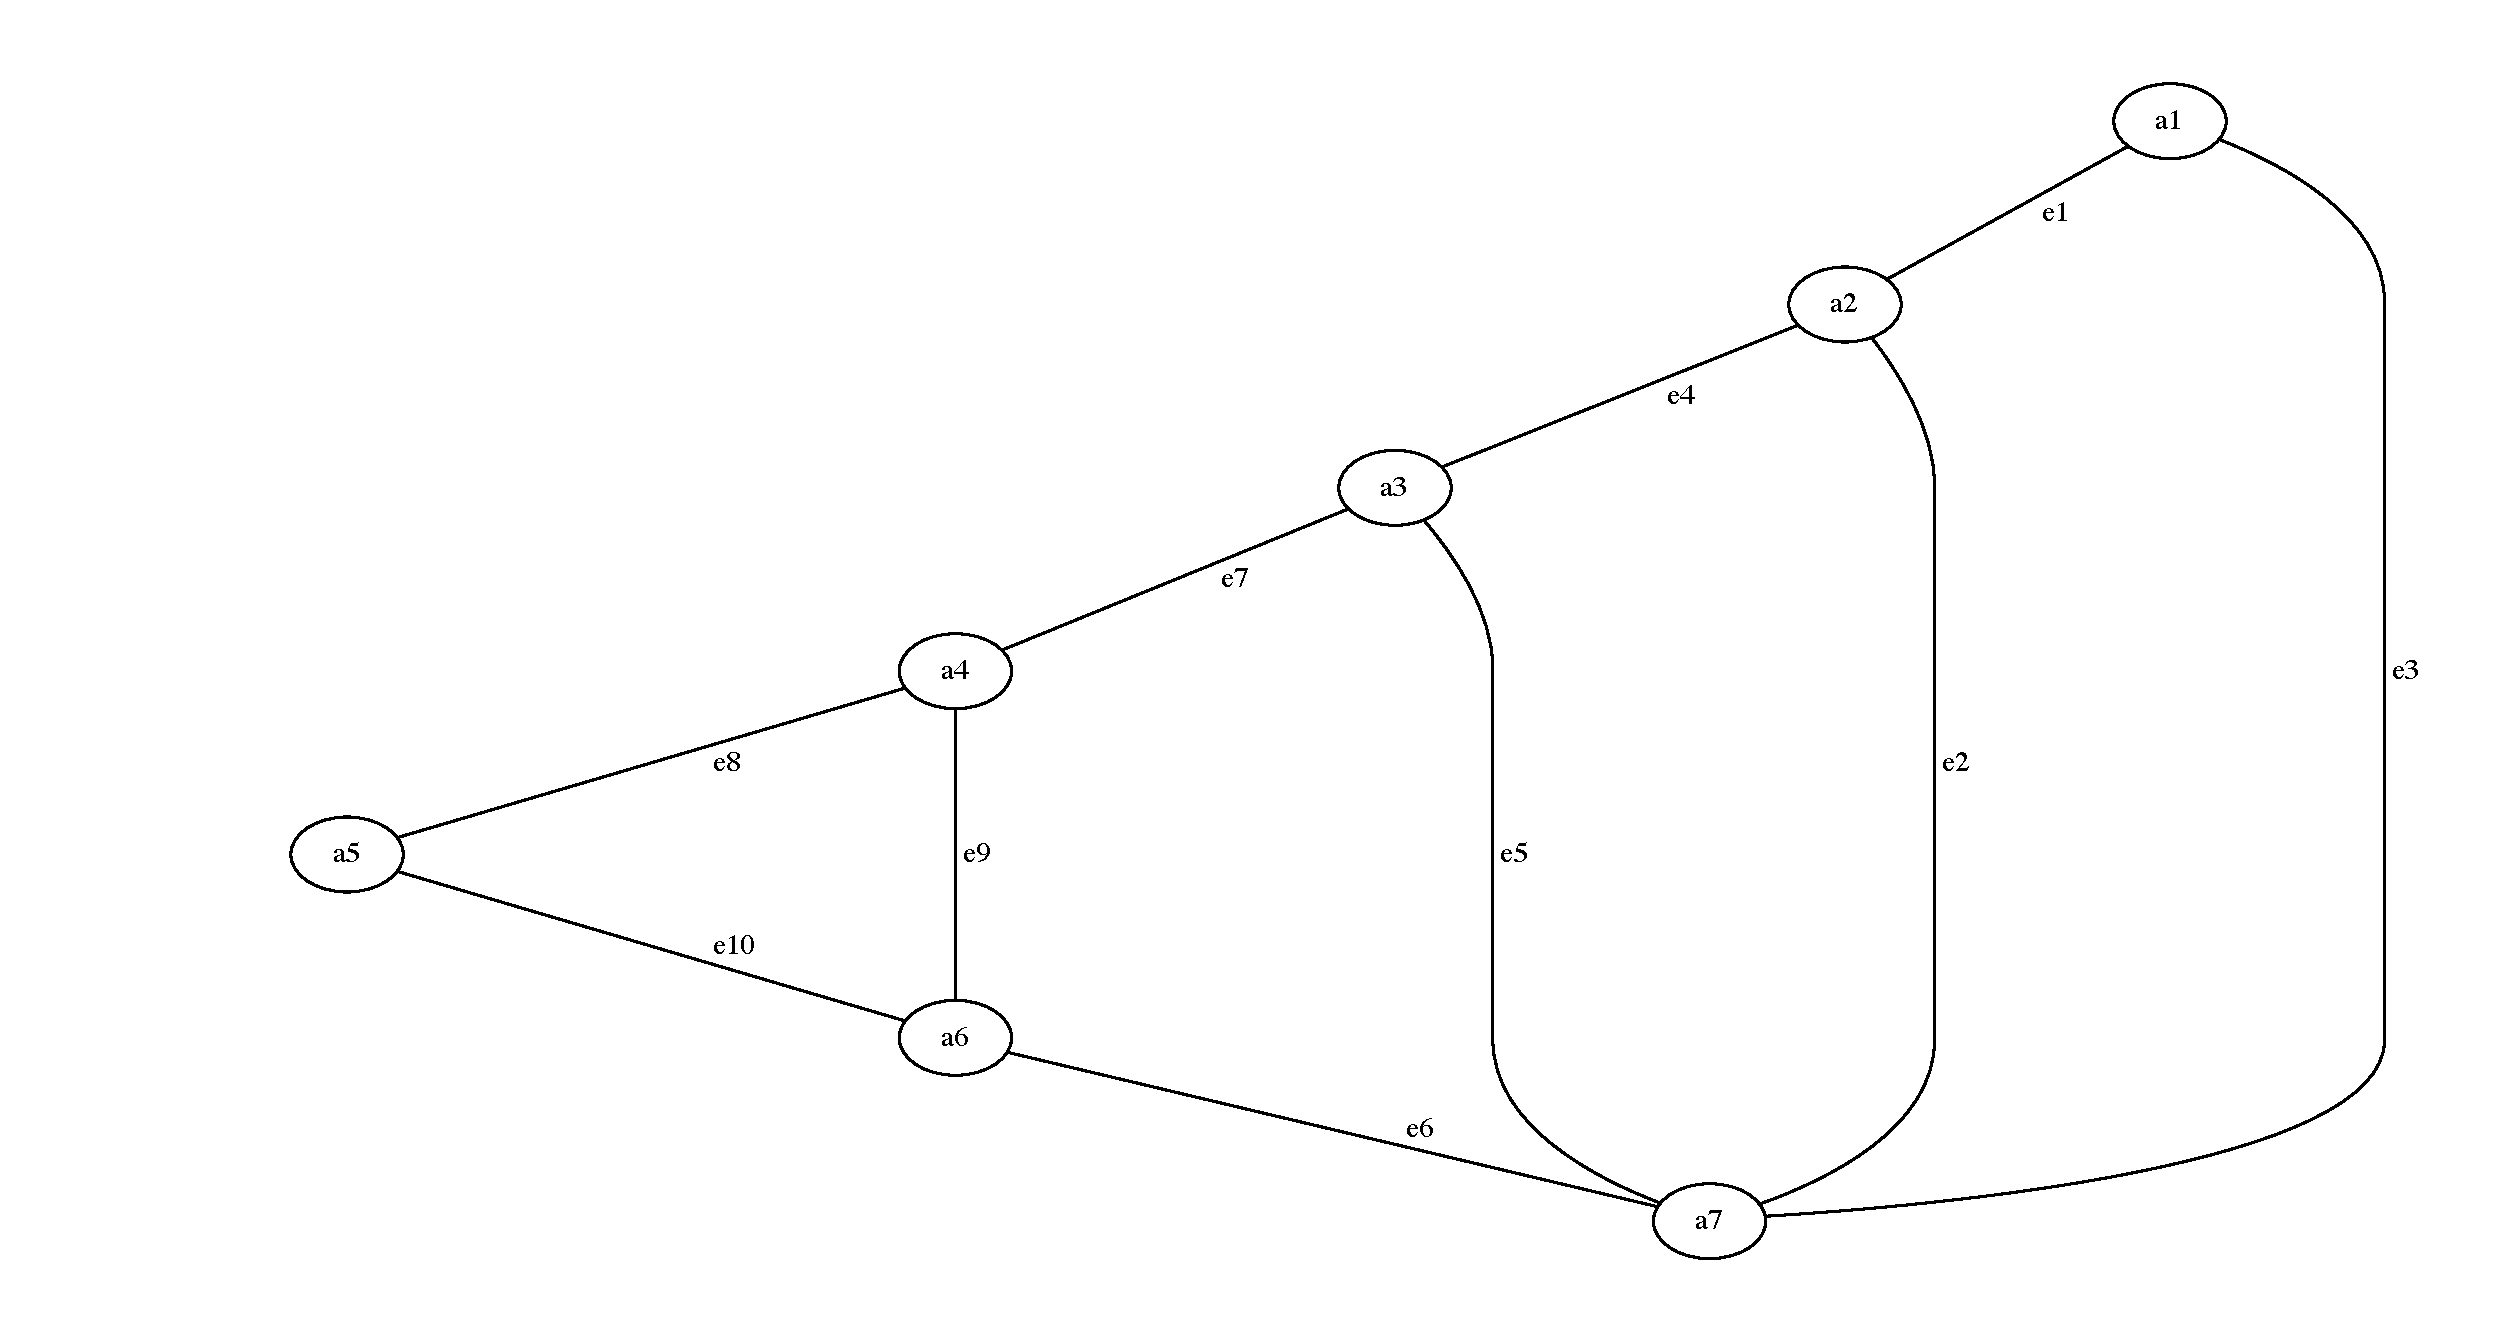
\includegraphics[scale=0.35]{diagrams/Chapter4_Example1.pdf}\\
\end{example*}
Remark: Perfect matching not possible with $\lvert V \rvert$ being odd. 
Maximum cardinality = 3. Empty set is a matching. All subsets of matchings are matchings.
\\
Maximum cardinality:
$\left\{e_{3},e_{1},e_{9}\right\}$
 $\left\{e_{10},e_{5},e_{1}\right\}$\\
Maximal matching:
$\left\{e_{2},e_{9}\right\}$
\begin{lemma}
If $M$ is a matching of maximum cardinality it is a maximal matching.
\end{lemma}
\begin{proof}
Let $M'$ be a matching with $M\subseteq M'$, assume $M \subset M'$ then $\lvert M' \rvert > \lvert M \rvert $ \Lightning (as $M$ has maximum cardinality).
\end{proof}
Remark: There are maximum matchings without maximum cardinality.
\begin{lemma}
If $M$ is perfect then $2 \lvert M \rvert = \lvert V \rvert$.
\end{lemma}
\begin{proof}
Obvious.
\end{proof}
\begin{lemma}
If a graph has a perfect matching $M$ then every matching of maximum cardinality is perfect. Clearly, $M$ is
of maximum cardinality.
\end{lemma}
\begin{proof}
Obvious.
\end{proof}
\section{Matching in bipartite graphs}\index{Matching in bipartite graphs}
Problem: Find a matching of maximum cardinality in a bipartite graph.\\
Solution: Construct an associated network as follows:\\
Let $G=(V,E)$ in a bipartite graph.\\ $V = X \cup Y$\\$\overline{V}=V \cup \left\{s,t\right\}$\\
$X\cap Y=\emptyset$\\$\overline{E}=\left\{s \rightarrow x: x \in X \right\}\cup \left\{ y \rightarrow t: y \in Y \right\}$\\
$\overline{c}(\overline{e})=1, \forall \overline{e} \in \overline{E}$
\begin{example*}
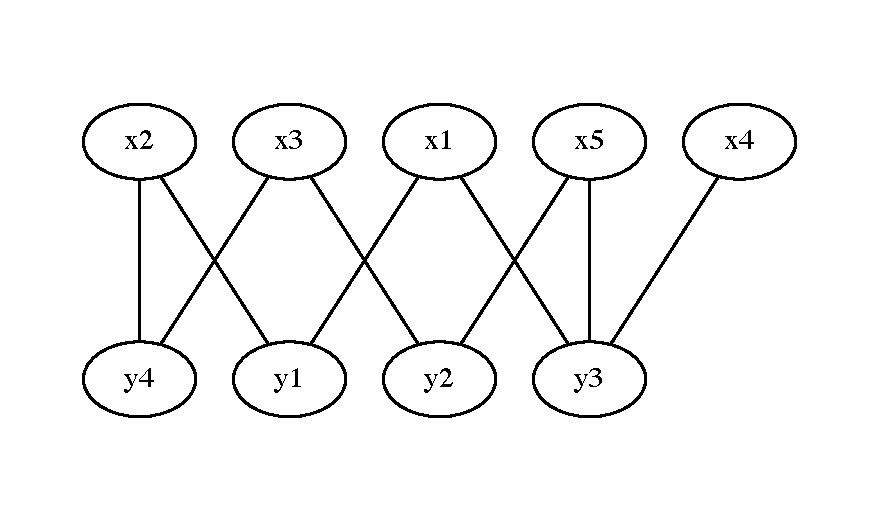
\includegraphics[scale=0.6]{diagrams/Chapter4_Example2.pdf}\\
One solution:\\
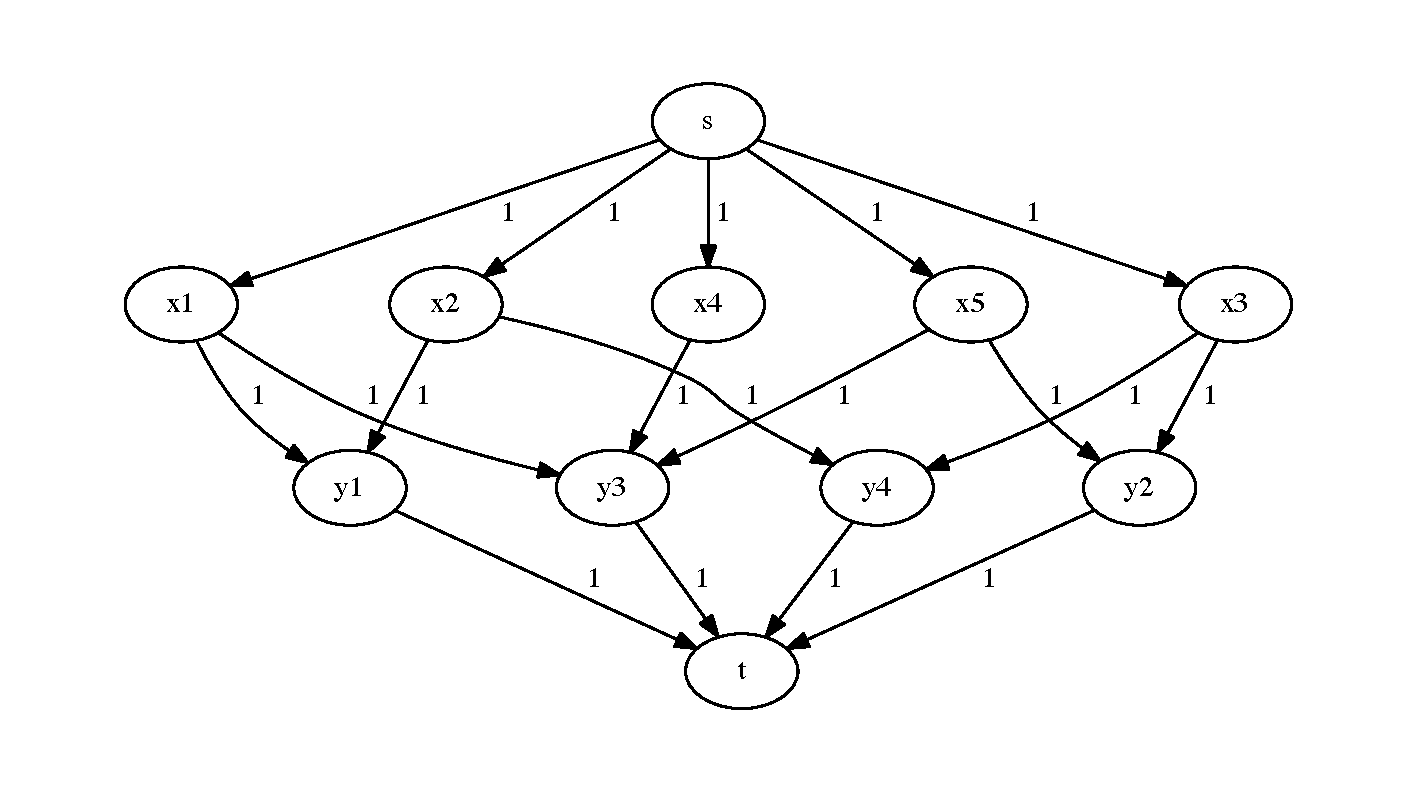
\includegraphics[scale=0.6]{diagrams/Chapter4_Example3.pdf}\\
\end{example*}
UNKLARHEIT IN NOTIZEN
\begin{theorem}
The number of edges in a matching $M$ of maximum cardinality coincides with $F_{max}$, i.e. the
 maximum total flow in the associated network.
\end{theorem}
\begin{proof}
Let $M$ be a matching of maximum cardinality. For every edge $x-y$ in $M$ we transport one unit along
the path $s-x-y-t$. We can do that as the edges in $M$ are node disjoint, i.e. they do not share nodes.
This defines a flow function $f'$ with $F'=\lvert M \rvert$ and hence $F_{max}\ge F' = \lvert M \rvert$. 
Now let $f$ be an arbitrary flow function for the associated network, without loss of generality we may choose
$f$ such that $f(e)\in \mathbb{N} \: \forall e$. All paths that connect $s$ with $t$ have the form 
$s \rightarrow x \rightarrow y \rightarrow t$. If such a path is used to transport a unit value then it is clear that
no flow can happen along edges of the form $x \rightarrow y'$ or $x' \rightarrow y$.
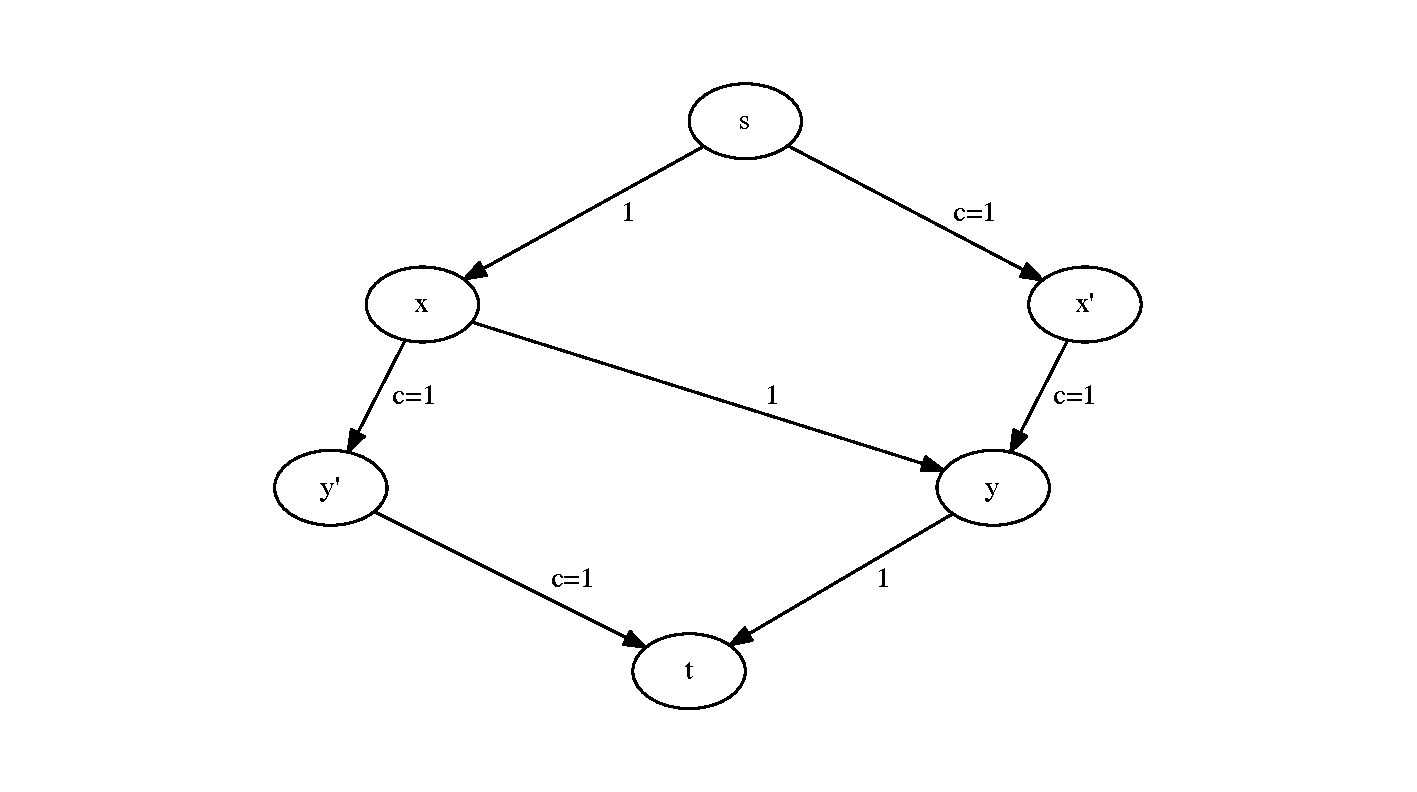
\includegraphics[scale=0.6]{diagrams/Chapter4_Example4.pdf}\\
Let $N=\left\{x-y:f(x \rightarrow y)=1\right\}$. $N$ is a matching and the total flow of $f$, i.e. $F$, satisfies
$F=\lvert N \rvert \le \lvert M \rvert$, hence also $F_{max}$, because $M$ was assumed to be of maximum cardinality.
Hence $\lvert M \rvert=F_{max}$ because we chose $f$ arbitrarily. 
\end{proof}
This theorem yields an algorithm to determine
a matching of maximum cardinality. Given a bipartite graph $G=(V,E)$ with $V = X \cup Y$ and $X \cap Y = \emptyset$:
\begin{enumerate}
  \item Construct the associated network.
  \item On this network, calculate a flow function with maximum total flow.
  \item The matching of maximum cardinality is obtained by $N=\left\{x - y: f(x \rightarrow y) = 1\right\}$.
\end{enumerate}
\begin{definition}
Let $G$ be a bipartite graph, $V = X \cup Y \: ; X \cap Y = \emptyset$. Let $A \subseteq X$. Let $\Gamma(A)=
\left\{y \in Y: \exists x \in A: x - y \in E\right\}$. ($\Gamma(A)$: potential partners for the elements in A).
A matching $M$ is called \emph{complete} if $\lvert M \rvert = \lvert X \rvert$, i.e. every $x \in X$ gets a partner.
\end{definition}
\begin{theorem}
Wedding or marriage theorem: A bipartite graph has a complete matching if and only if for every $A \subseteq X$
$\lvert \Gamma(A) \rvert \ge \lvert A \rvert$.
\end{theorem}
\begin{proof}
``>'' Let G have a complete matching $M$, let $A \subseteq X$. Then every $x \in X$ has a partner for itself in $M$,
hence for every $A \subseteq X \lvert \: \Gamma(A) \rvert\ge \lvert A \rvert$. \\
``<'' Let $\lvert \Gamma (A) \rvert \ge \lvert A \rvert$ for every $A \subseteq X$. Assume there is no complete
matching. Let $S$ be the set of nodes that were marked in the last step of Ford-Fulkerson in the associated 
network. The calculated flow function determines a matching $M$ with i) $F=\lvert M \rvert$. As we assumed that there
is no complete matching we get ii) $\lvert M \rvert < \lvert X \rvert$.\\
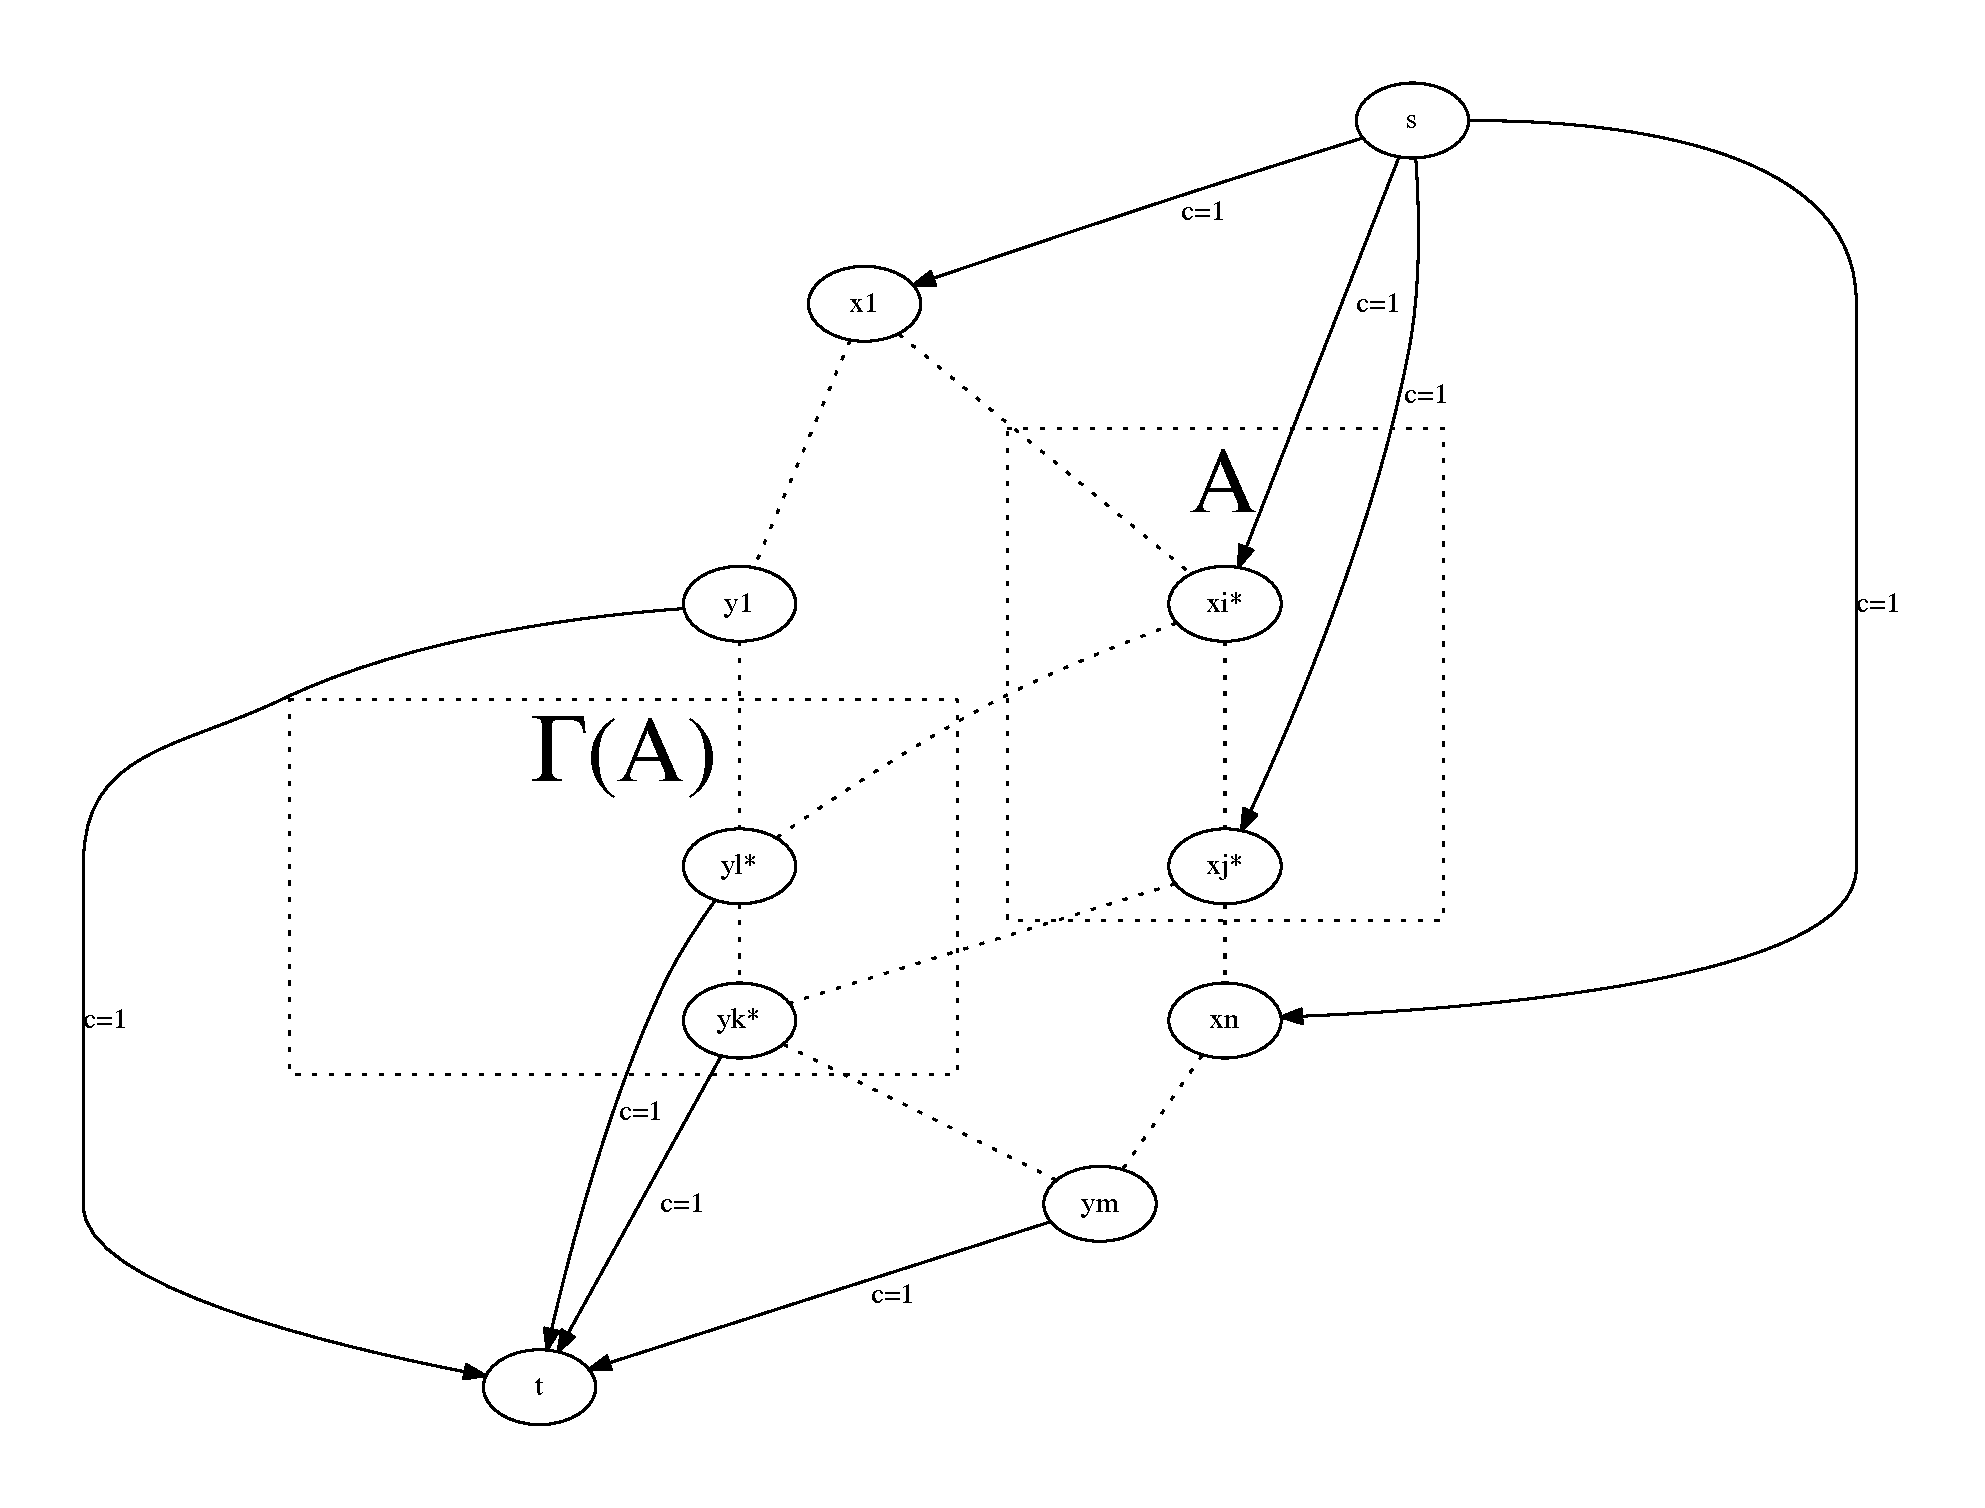
\includegraphics[scale=0.45]{diagrams/Chapter4_Example5.pdf}\\
Marking in the last round of Ford-Fulkerson. $S=$ the marked nodes.\\
$A:=X \cap S$\\
Let $y \in \Gamma (A)$ then there is an $x \in A = \: X \cap S \: x$ marked and $x-y$ is an edge in $E$. <- NOTIZEN UNKLAR \\
In the last successfull construction of an augmenting path there was no flow determined along the edge $s \rightarrow x$,
otherwise we could not mark $x$ now. Hence the flow along the edge $x \rightarrow y$ must have been $0$ before 
as well. Hence the remaining capacity $x \rightarrow y \: = 1$.
\section{Stable matching (marriage)}\index{Stable matching (marriage)}
Given:\\ 
1. n men $b_{1} \dots b_{n}$, n women $a_{1} \dots a_{n}$\\
2. each person has a preferene list of the other sex: \\
$a_{1}: b_{2}, b_{3}, b_{1} \dots$, where $a_{1}$ likes $b_{2}$ best.
\end{proof}